\usetikzlibrary{arrows.meta}
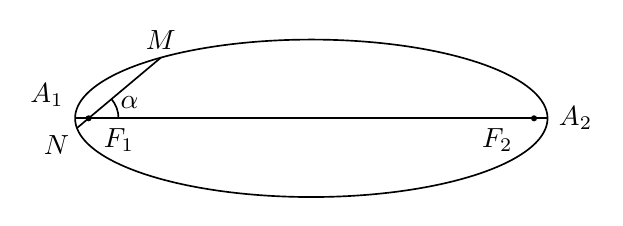
\begin{tikzpicture}[x=1cm,y=1cm,line width=.6pt,font=\normalsize,>=Stealth,
  axis/.style={->,line width=.6pt},curve/.style={line width=.6pt},segment/.style={line width=.6pt},label/.style={inner sep=1pt}]
\def\ea{3}
\def\eb{1}
\coordinate (A1) at (-3.0,0.0);
\coordinate (A2) at (3.0,0.0);
\coordinate (F1) at (-2.828427,0.0);
\coordinate (F2) at (2.828427,0.0);
\coordinate (M) at (-1.909136,0.771377);
\coordinate (N) at (-2.976693,-0.12441);
\draw[curve] plot[domain=0:360,samples=240] ({\ea*cos(\x)},{\eb*sin(\x)});
\draw[segment] (A1)--(A2);
\draw[segment] (M)--(N);
\fill (F1) circle (1.1pt);
\fill (F2) circle (1.1pt);
\draw[segment] ([shift={(0.38,0)}]F1) arc[start angle=0,end angle=40,radius=0.38];
\node[label,anchor=south east] at (-3.1,0.1) {$A_1$};
\node[label,anchor=west] at (3.1,0.0) {$A_2$};
\node[label,anchor=north west] at (-2.68,-0.08) {$F_1$};
\node[label,anchor=north east] at (2.6,-0.08) {$F_2$};
\node[label,anchor=south] at (-1.91,0.83) {$M$};
\node[label,anchor=north east] at (-3.03,-0.18) {$N$};
\node[label,anchor=center] at (-2.31,0.2) {$\alpha$};
\end{tikzpicture}
